\begin{figure}[!h]
	\begin{subfigure}{\linewidth}
		\caption{\label{fig:var_receita_despesa_primaria}Variação da receita e despesa primária}
		\subcap{Variação acumulada (base: igual período do ano anterior)}
		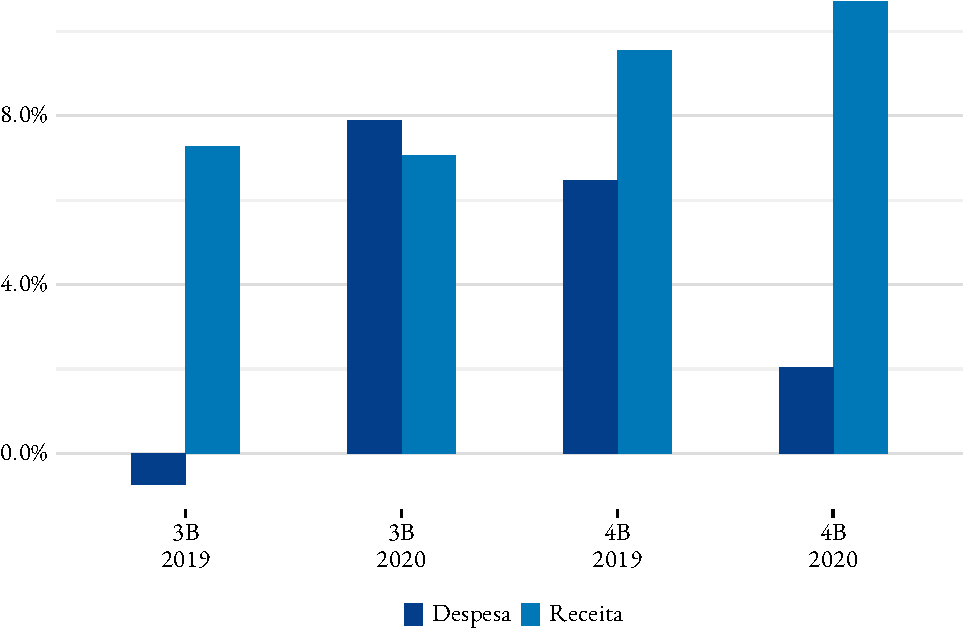
\includegraphics{fig/var_receita_despesa_primaria-1.pdf}
		\source{\abbr{siconfi}/Tesouro Nacional}
		\notes{\bimestres[3-4]}
	\end{subfigure}
	\begin{subfigure}{\linewidth}
		\caption{\label{fig:var_despesa_categoria}Variação da despesa por categoria}
		\subcap{Variação acumulada (base: igual período do ano anterior)}
		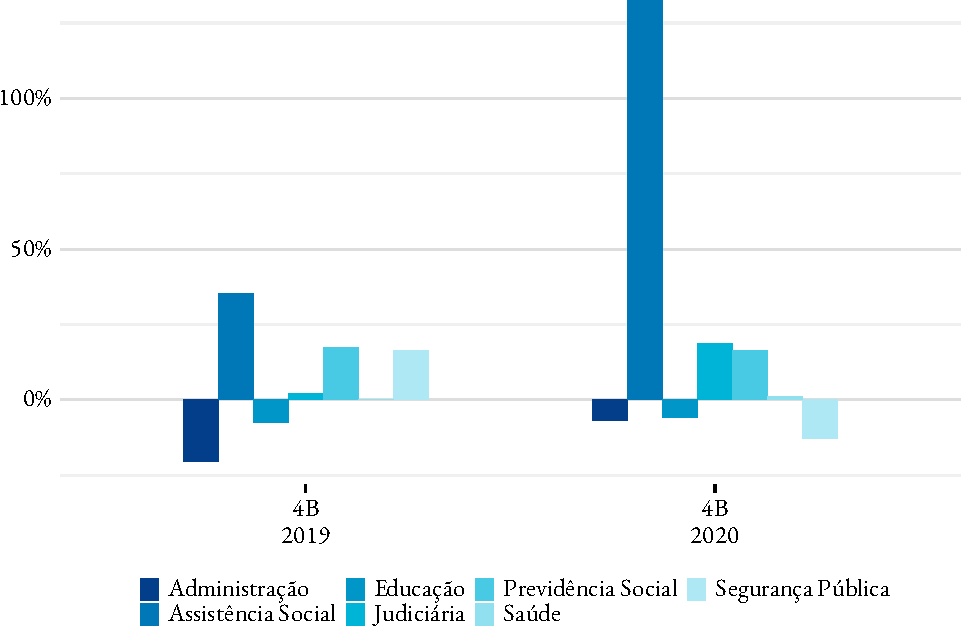
\includegraphics{fig/var_despesa_categoria-1.pdf}
		\source{\abbr{siconfi}/Tesouro Nacional}
		\notes{\bimestres[4]}
	\end{subfigure}
	\begin{subfigure}{\linewidth}
		\caption{\label{fig:desp_pessoal_rcl}Despesa total com pessoal em relação à RCL}
		\subcap{RCL e despesa acumulada até agosto}
		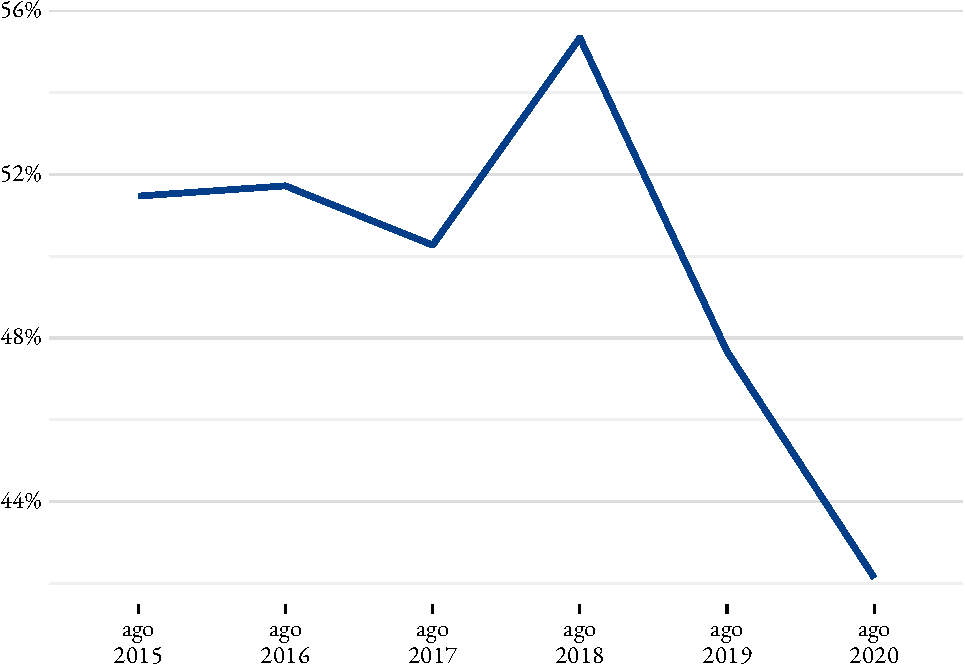
\includegraphics{fig/desp_pessoal_rcl-1.pdf}
		\source{\abbr{siconfi}/Tesouro Nacional}
	\end{subfigure}
\end{figure}


\begin{figure}[!h]
	\begin{subfigure}{\linewidth}
		\caption{\label{fig:divida_rcl}Dívida Consolidada Líquida em relação à RCL}
		\subcap{RCL e DCL acumulada até agosto}
		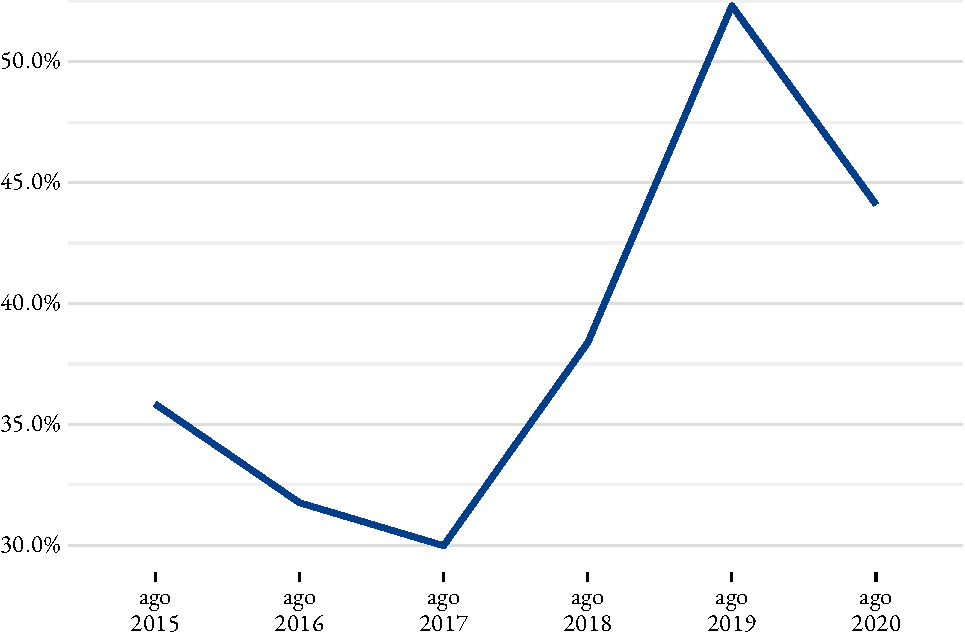
\includegraphics{fig/divida_rcl-1.pdf}
		\source{\abbr{siconfi}/Tesouro Nacional}
	\end{subfigure}
\end{figure}

\begin{table}[!h]
	\caption{\label{tab:capag}Nota da capacidade de pagamento}
		\subcap{Indicadores da CAPAG}
	\begin{tabu} to \linewidth {>{\raggedright}X>{\centering}X>{\centering}X>{\centering}X>{\centering}X>{\centering}X>{\centering}X}
	\toprule
	\multicolumn{1}{c}{ } & \multicolumn{2}{c}{Endividamento} & \multicolumn{2}{c}{\makecell[c]{Poupança\\Corrente}} & \multicolumn{2}{c}{Liquidez} \\
	\cmidrule(l{3pt}r{3pt}){2-3} \cmidrule(l{3pt}r{3pt}){4-5} \cmidrule(l{3pt}r{3pt}){6-7}
	UF & 2019 & 2020 & 2019 & 2020 & 2019 & 2020\\
	\midrule
	AC & B & B & B & B & A & A\\
	AM & A & A & B & B & A & A\\
	AP & B & B & A & A & A & -\\
	PA & A & A & B & B & A & A\\
	RO & B & A & A & A & C & A\\
	\addlinespace
	RR & A & A & A & A & C & C\\
	TO & A & B & B & C & C & C\\
	\bottomrule
	\end{tabu}
		\source{Boletim de Finanças dos Entes Subnacionais, 2019–-2020/Tesouro Nacional}
		\notes{Amapá teve nota suspensa}
	\end{table}
